\chapter{State of Art}
%%%%%% SLEEP STAGES %%%%%%
\section{Sleep Stages} \label{cap:sleepStages}
\begin{comment}
For this reason, it is nowadays 
acceptable to use cardiorespiratory polysomnography that does not track neurophysiological variables. This type of polysomnography
involves a cannula, chest belts and electrodes for an electrocardiogram (ECG) but does not involve an electroencephalogram (EEG).
Another reason why this kind of instrument is widely used is that inside the population, we have a higher percentage of 
sleep-related breathing disorders that can be studied and monitored with this instrument, like sleep apnoea/hypopnoea syndrome (SAS), 
where the individuals experience a collapse 
of the airway in deeper sleep states. The ability to monitor it allows for a faster and closer intervention in severe cases. \end{comment}

Sleep is a fundamental physiological function that occupies one-third of everyday life and affects almost every type of tissue and system in the body from the brain, heart, and lungs to metabolism, immune function, mood, and disease resistance. The quality and the quantity also can affect mental wellness, for example, lack of sleep affects our memory and ability to think clearly or sleep deprivation can lead to neurological dysfunction such as hallucinations. Moreover, those who do not get enough sleep are at higher risk of developing high blood pressure, cardiovascular disease, diabetes, depression, and obesity \cite{Colten2006SleepProblem}.

The sleep cycle of a person is divided into two phases Non-Rapid Eye Movement (NREM) and Rapid Eye Movement (REM); 
this second phase is further divided into three other stages (N1-N3). 
Different muscle tones, brain wave patterns, eye movements, and heart and breathing rate alterations characterise every phase and stage. Each cycle is approximately 90 minutes long, over the course of the night a person goes through four to six 
sleep cycles\cite{Patel2022PhysiologyStages}. The composition of each cycle, so time spent in each sleep stage, changes as the night goes along and depending on other factors such as age, recent sleep patterns, and alcohol consumption. 
During an interrupted sleep, the stages progress as follows, also visible in Fig \ref{diag:slepcy}:
\begin{itemize}
    \item Awake to NREM stage 1 sleep.
    \item NREM stage 1 progresses into NREM stage 2.
    \item NREM stage 2 is followed by NREM stage 3.
    \item NREM stage 3 to REM sleep.  
\end{itemize}

Then the cycle comes back to NREM stage 1.
\vspace*{1.0cm}

\begin{figure}[H]
    \begin{center}
        \begin{tikzpicture}[node distance=4cm]
            %% nodi:
            \node (inizio) [box] {Awake};
            \node (stage1) [box, right of=inizio] {NREM\\Stage 1};
            \node (stage2) [box, right of=stage1] {NREM\\Stage 2};
            \node (stage3) [box, above of=stage2] {NREM\\Stage 3}; 
            \node (rem) [box, left of=stage3] {REM}; %yshift=-3cm
            %yshift=-1cm
            \draw [arrow] (inizio) -- (stage1);
            \draw [arrow] (stage1) -- (stage2);
            \draw [arrow] (stage2) -- (stage3);
            \draw [arrow] (stage3) -- (rem); % node[anchor=east] {Yes} 
            %\draw [arrow] (quest) -- ++(4,0) -- ++(0,5) -- node[] {No} (if_1);
            \draw [arrow] (rem) -- (stage1);
        \end{tikzpicture}
    \end{center}
    \caption{Sleep Cycles}
    \label{diag:slepcy}
\end{figure}
\vspace*{1.0cm}

\begin{comment}
\begin{figure}[H]
    \centering
    %\smartdiagram[flow diagram:horizontal]{NREM stage 1, NREM stage 2, NREM stage 3, REM}
        \caption{Sleep Cycles}
    \label{diag:slepcy}
\end{figure}
\end{comment}

NREM sleep is composed of three stages \cite{StagesFoundation}:
\begin{itemize}
    \item N1: the first stage happens when a person first falls asleep, it last between one and seven minutes. The body has not fully relaxed and body and brain activities start to slow with periods of brief movements. If there are no external events a person can go into stage 2, during the night an uninterrupted sleeper may not spend much more time in stage 1 as they move through further sleep cycles.
    \item N2: During the second stage the body has a drop in temperature,  muscles start to relax, and slowed breathing and heart rate. Simultaneously, brain activity slows, even if they still present some short bursts of activity and eye movement stops. This stage can last for 10 to 25 minutes during the first sleep cycle, and each N2 stage can become longer during the night. Jointly, half of the sleep time is in N2 sleep.
    \item N3: The last stage of NREM or deep sleep is when the body is more relaxed: muscle tone, pulse and breathing rate decrease.
    The brain activity during this period has an identifiable pattern of what is known as delta waves. For this reason, stage 3 may also be called delta sleep or slow-wave sleep (SWS). This stage is critical for restorative sleep, allowing for the body to recover and grow. Even though brain activity is reduced, there is evidence that deep sleep contributes to insightful thinking, creativity, and memory\cite{Yordanova2010DifferentialRegularity}. The duration of this stage is 20 to 40 minutes, overnight the other stages became shorter and more time gets spent in REM sleep instead.
\end{itemize}

REM sleep is characterised by brain activity near levels of awakeness, due to this at the same time the body experience atonia, which is a temporary paralysis of the muscles, with two exceptions: the eyes and the muscles that control breathing. Even though the eyes are closed, they can be seen moving quickly, which is how this stage gets its name.
This sleep phase is essential to cognitive functions like memory, learning, creativity and emotions \cite{Baran2012ProcessingSleep}.
REM sleep is known for the most vivid dreams, which is explained by the significant uptick in brain activity, this is why the body experiences a temporary atonia as it prevents from acting out inside dreams. Dreams can occur in any sleep stage, but they are less common and intense in the NREM periods. The first REM stage could last only a few minutes, and later stages can last for around an hour.

Both NREM and REM are important because they allow the brain and body to recuperate and develop. Sleepers who are frequently awoken during earlier stages, such as people with sleep apnea, may struggle to properly cycle into these deeper sleep stages. People with insomnia may not get enough total sleep to accumulate the needed time in each stage.


%%%%%% RESPIRATORY SYSTEM %%%%%%
\section{Respiratory System} \label{cap:respiratorySystem}

Respiration is the physiological process\cite{FISHER1983223} of our body to exchange carbon dioxide (CO$_2$) with oxygen (O$_2$). This process has an external phase that consists of the exchange of gases with the environment and the transfer of gas across the blood-gas barrier, and an internal phase that begins with the loading of oxygen onto the haemoglobin molecule and is followed by the transportation, delivery, and transfer of O$_2$ to the tissue. CO$_2$ is delivered back to the lung and ventilated out to the environment with the reversed process.

Normal tidal breathing is comprised of inspiratory and expiratory phases and occurs with the synchronous movement of the thorax and abdomen.
In particular, during inhalation (Fig.\ref{fig:resp}.a ), when we have the loading of O$_2$ into haemoglobin, the diaphragm moves downward toward the abdomen, and the rib muscles pull the ribs upward and outward making the chest cavity bigger and pulling air through the nose or mouth into the lungs. In exhalation,(Fig.\ref{fig:resp}.b), when the CO$_2$ leave the body, the diaphragm moves upward and the chest wall muscles relax, causing the chest cavity to get smaller and push air out of the respiratory system through the nose or mouth.

This movement can be automatic or can be controlled voluntarily and it is adjusted based on the activity performed at that moment like coughing, sneezing, yawning, or speaking if a person is eating it is coordinated to chew and swallow to avoid choking. It could also increase as a response to physical activity, like running or climbing stairs\cite{DelNegro2018BreathingMatters}.\\

\vspace{0.6cm}
\begin{figure}[H]
    \centering
    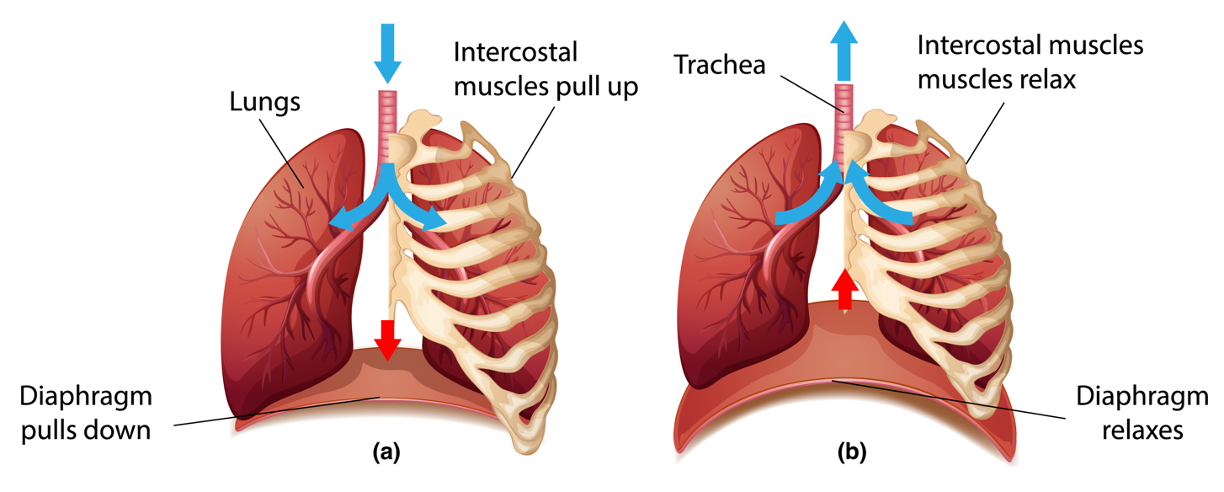
\includegraphics[width=\textwidth]{img/j338_ps1n_201111.png}
    \caption{Respiratory sistem}
    \label{fig:resp}
\end{figure}
\vspace{0.7cm}


The respiration and the tidal volume vary in response to metabolic demand or diseases such as infection. Patients with elevated respiratory rates, reflected by the magnitude of the metabolic demand, often have a more serious illness. 

The respiratory rate per minute (rpm) varies by age, focusing on healthy adults the average respiratory rate at rest is between 12 and 15 breaths per minute\cite{barrett2010ganong}.

Some studies found that a respiratory rate greater than 20 breaths per min was predictive of cardiopulmonary arrest within 72 hours and death within 30 days\cite{Hong2013HowPatients}; greater than 27 breaths per minute was predictive of cardiopulmonary arrest within 72 hours \cite{Fieselmann1993RespiratoryInpatients}; also a prospective observational study of acute medical admissions, patients with a composite outcome of cardiopulmonary arrest, intensive care admission, or death within 24 hours had a mean respiratory rate of 27\cite{Subbe2003EffectAdmissions}.

%%%%%% POLYSOMNOGRAPHY %%%%%%
\section{Polysomnography} \label{cap:POLYSOMNOGRAPHY}

Polysomnography (PSG) is the state-of-art to monitor physiological data during sleep and is used to diagnose sleep disorders \cite{Penzel2016ModulationsPolysomnography, RUNDO2019381}, such as obstructive sleep apnea (OSA), sleep-related hypoventilation/hypoxia, nocturnal seizure, or periodic limb movement disorder. PSG require a complex monitor system because it consists of several instruments that the patient has to wear, visible in Fig \ref{fig:PSGComplete}.

This procedure involves:
\begin{itemize}
    \item electroencephalogram(EEG)\cite{ElectroencephalogramMedicine}: this test measures electrical activity in the brain using electrodes, small metal discs with wires pasted on the scalp.
    \item electrooculogram(EOG)\cite{CREEL2019495}: this test measures the corne-positive stain potential relative to the back of the eye, it is performed using skin electrodes outside the eye.
    \item electromyogram(EMG)\cite{ElectromyographySite}: this diagnostic procedure can reveal nerve dysfunction, muscle dysfunction or problem with nerve-to-muscle signal transmission since is used to assess the health of muscles and the nerve cells that control them.
    \item electrocardiogram(ECG)\cite{ElectrocardiogramNHS}: this test can be used to check the heart's rhythm and electrical activity.
    \item pulse oximetry\cite{PulseMedicine}: this electronic device measures the saturation of oxygen carried in red blood cells, it is used to understand how well the oxygen is being sent to the part of the body furthest from the heart.
    \item cannula: this instrument via nasal pressure monitor the airflow and respiratory effort\cite{heitman2002validation}.
    \item respiratory inductance plethysmography(RIP)\cite{Brullmann2010RespiratoryCalibration}: which is a method of evaluating pulmonary ventilation by measuring the movement of the chest and abdominal wall.
\end{itemize}
As part of PSG are also monitored limb movement, body position and as derived data sleep stages. 
After the test is completed a ``score" analyzes the data by 30-second ``epochs".

\begin{figure}[p]
    \centering
    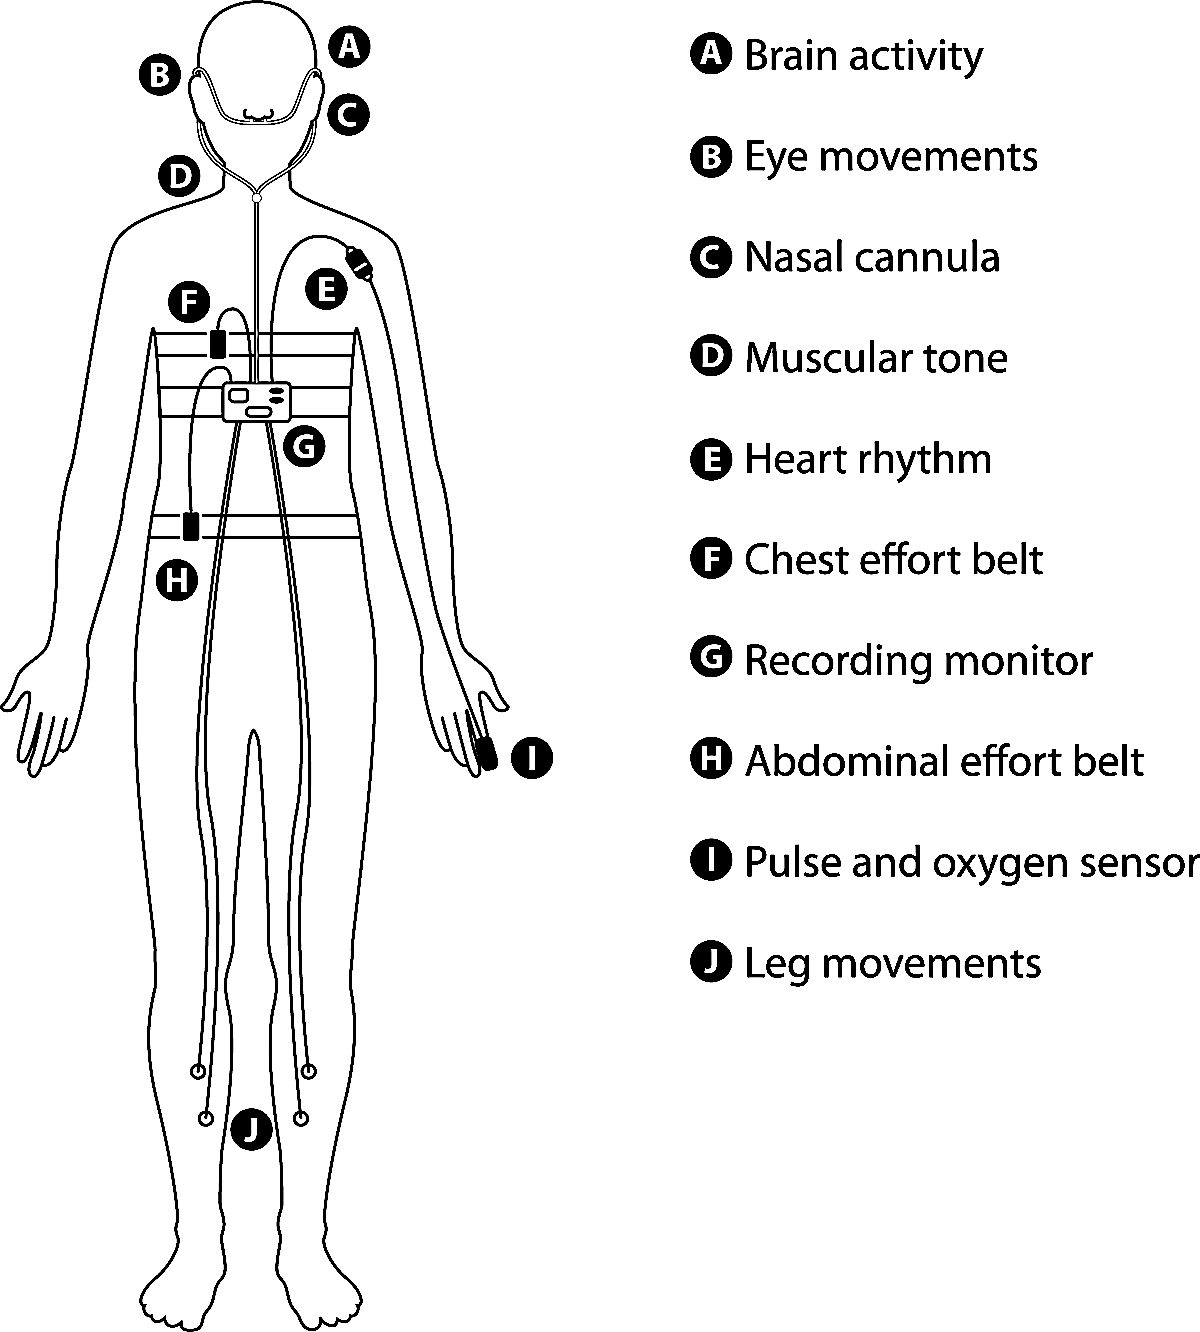
\includegraphics[width=\textwidth]{img/PSG test.png}
    \caption{Polysomnography}
    \label{fig:PSGComplete}
\end{figure}

%%%%%% CARDIO RESPIRATORY %%%%%%
\subsection{Cardiorespiratory Polysomnography} \label{cap:cardiorespiratory}
The state-of-the-art to monitor physiological data during sleep is polysomnography (PSG) \cite{Penzel2016ModulationsPolysomnography}, described in Chapter (\ref{cap:POLYSOMNOGRAPHY}, which involves recording sleep stages, respiratory rate, heart and other parameters. However, this procedure is time-consuming, complicated, expensive, invasive for the patient and only sometimes available in hospitals. 
%\textbf{[explenation of sleep stages]}.
Focusing on sleep-related breathing disorders, like sleep apnoea/hypopnoea syndrome (SAS), there is the possibility to use cardiorespiratory polysomnography instead of full PSG. This type of PSG involves fewer instruments, as shown in Figure\ref{fig:PSGCardio}, and in particular, does not record neurophysiological variables avoiding using EEG electrodes that can cause high discomfort for the patient.  
Even if this method compared to full PSG can collect less parameters, it is used to diagnose SAS \cite{Calleja1505} and Obstructive sleep apnea(OSA) and other breath-related disturbs or also to track the effectiveness of other treatments during sleep.

Focusing on one of the vital signs that characterise the different sleep stages, respiratory rate (as discussed in Chapter \ref{cap:sleepStages}). It is described by becoming slowly and more stable going from the awake to the REM phase and increasing its rate going to the NREM phase.
This fluctuation characterizes the different stages and gives the possibility to understand in which stage a person is based on the parameter extracted via cardiorespiratory PSG \cite{7318373}, such as respiratory inductance plethysmography and nasal pressure. In some studies, the sleep stages, are often classified using a combination of respiratory signals and heart rate \cite{1597499}, that cardiorespiratory PSG monitor.

This instrument is increasingly used in a medical context, for the reasons mentioned above and because cardiorespiratory PSG devices are
becoming smaller and more portable, such as NOX A1 described in Chapter\ref{cap:NOXA1}, with accuracy and user-friendliness that allow being used in a home environment.

\vspace{0.5cm}
\begin{figure}[h]
    \centering
    \includegraphics[width=\textwidth]{img/CardioPSG.jpg}
    \caption{CaridiorespiratoryPolysomnography}
    \label{fig:PSGCardio}
\end{figure}

%%%%%% PRESSURE SENSOR MATTRESS %%%%%%
\section{Unobstrusive sensors} \label{cap:unobstrusiveSensors}

As said before, the state-of-art is a cumbersome device that requires cables attached to the users' bodies and often interferes with natural sleep. To avoid it, in literature is possible to find new instruments such as video cameras, which lead to privacy concerns; radar technology, which could have problems in case there are more than one person inside the room; or smartwatches, which are also able to track respiratory rate but involve to have something on the arm that for some person can lead to discomfort.
\newline
The research field focused on discovering unobtrusive sensors to track vital signs proposed bed pressure sensors as a possible solution to these concerns. 
The pressure sensors used today are different and with different kinds of sensors like piezo-electric, inductive and capacitive. As an instrument, in literature is possible to find: pneumatic sensor array \cite{Holtzman2010ValidationEnvironments}, as shown in Figure\ref{fig:sensorArray}, that can be placed between the mattress and the box spring; micro bend optic fiber sensors mattress \cite{Sadek2017NonintrusiveStudy}, shown in Figure\ref{fig:sadek}, that are small, lightweight and affordable and also immune to electromagnetic and radio frequency interference, that can be placed directly under body's person; air-mattress \cite{articleAir}, shown in Figure\ref{fig:airmat}, that measure changes in air pressure inside single air comportment of an inflatable mattress.


\begin{figure}[h]
    \centering
    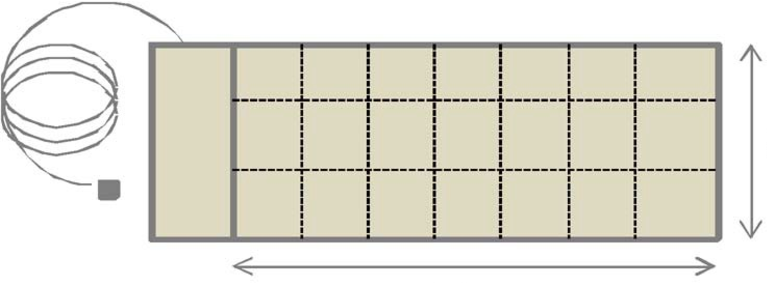
\includegraphics[width=0.7\textwidth]{img/pressure_array.pdf}
    \caption{Pressure Sensor Array}
    \label{fig:sensorArray}
    
\end{figure}
%\vspace*{0.5cm}
\begin{figure}[h]
   \centering
    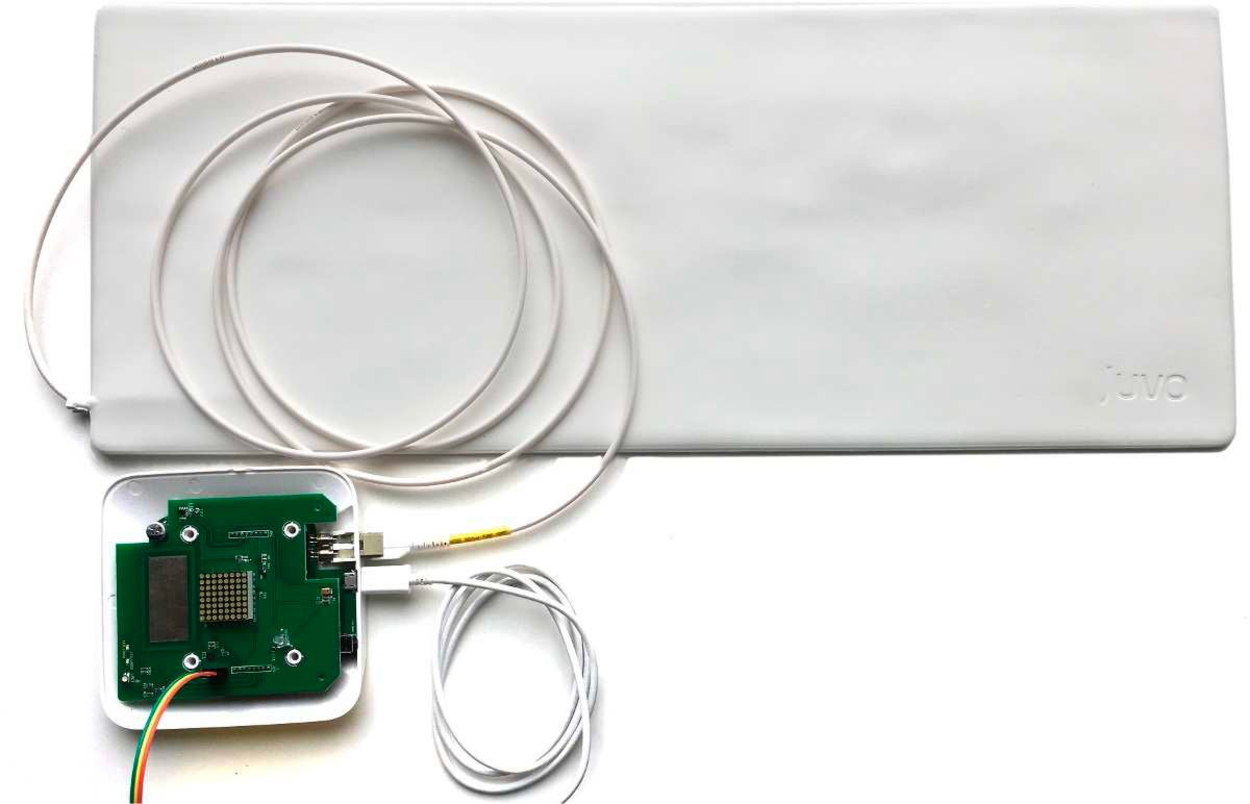
\includegraphics[width=0.6\textwidth]{img/sadek_fig.pdf}
    \caption{Sensing Mat (optic fiber sensors)}
    \label{fig:sadek}
\end{figure}
\begin{figure}[h]
    \centering
     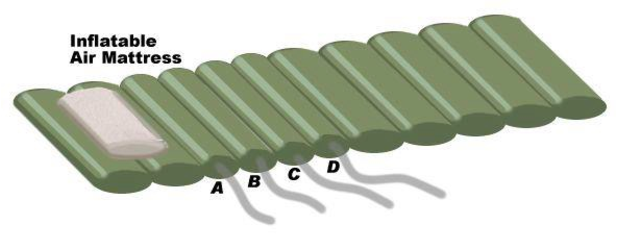
\includegraphics[width=0.7\textwidth]{img/arimat.pdf}
     \caption{Inflatable Mattress}
     \label{fig:airmat}
 \end{figure}


%%%%%% TEXTILE SENSOR MATTRESS %%%%%%
\subsection{Textile Pressure Mattress} \label{cap:textile}
A particular type of pressure mattresses available nowadays are textile pressure sensor mattresses, based on piezoelectric sensor, where each sensor appears as shown in Figure\ref{fig:sensomativeSensors}. This project involved two of these kinds of mattresses: Sensomative\cite{sensomativeUrl} described in Chapter\ref{cap:SensomativePar} and SensingTex\cite{SensingConnectivity} described in Chapter\ref{cap:SensigTexPar}.

These particular sensor mattresses appear like thin mattresses similar that can be easily installed with adjustable straps over a standard mattress. 
Due to their small height, they are completely unobtrusive and allow to monitor of both physiological and positional data without interfering with the patient's comfort.

\vspace{0.5cm}
\begin{figure}[h]
    \centering
     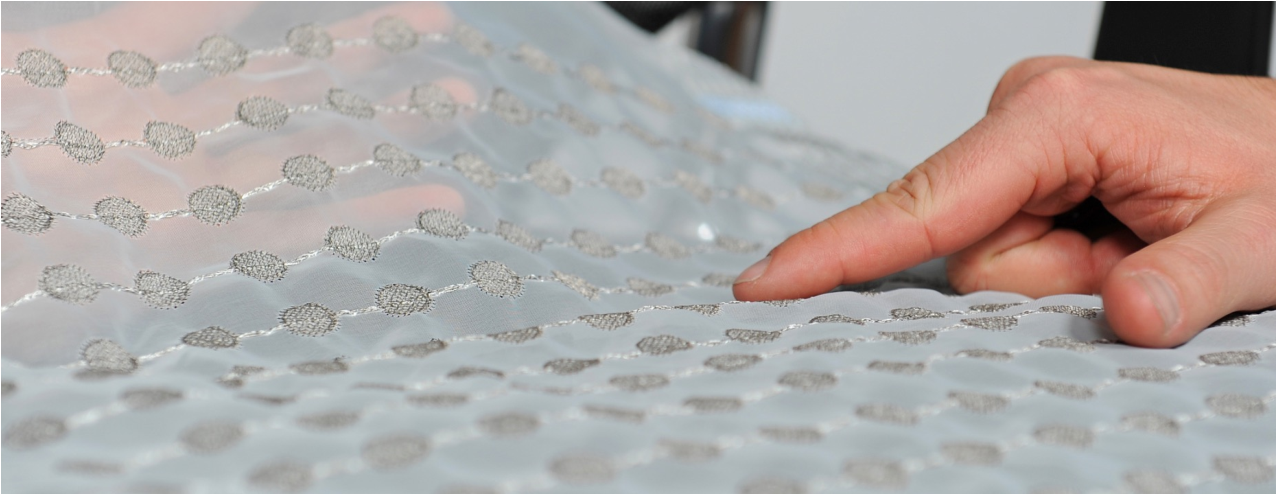
\includegraphics[width=0.9\textwidth]{img/sensomative.pdf}
     \caption{Sensomative textile sensors}
     \label{fig:sensomativeSensors}
 \end{figure}


\begin{comment}

%%
    Sleep is one of the most important physiological functions. Sleep quality can affect physical 
    and mental wellness; for this reason,
    it is crucial to monitor vital signs without interfering with natural sleep. 
    The state-of-the-art to monitor physiological data during sleep is polysomnography \cite{Penzel2016ModulationsPolysomnography}
    , which involves recording sleep stages, respiratory rate, heart and other parameters. However, this procedure is time-consuming, 
    complicated, expensive, invasive for the patient and only sometimes available in hospitals. For this reason, it is nowadays 
    acceptable to use cardiorespiratory polysomnography that does not track neurophysiological variables. 
    This type of polysomnography
    involves a cannula, chest belts and electrodes for an electrocardiogram (ECG) but does not involve an electroencephalogram (EEG).
   
    Another reason why this kind of instrument is widely used is that inside the population, we have a higher percentage of 
    sleep-related breathing disorders that can be studied and monitored with this instrument, like sleep apnoea/hypopnoea syndrome (SAS), 
    where the individuals experience a collapse 
    of the airway in deeper sleep states. The ability to monitor it allows for a faster and closer intervention in severe cases. 
    The sleep cycle of a person is divided into two phases Non-Rapid Eye Movement (NREM) and Rapid Eye Movement (REM);
    this second phase is further divided into three other stages (N1-N3). Different muscle tones, brain wave patterns, 
    eye movements, and heart and breathing rate alterations characterise every phase and stage.
    %\textbf{[explenation of sleep stages]}.
    Focusing on one of the vital signs that characterise the different sleep stages is the respiratory rate 
    which slowly becomes more stable going from the awake to the REM phase; this characterisation of the different stages gives the possibility to 
    understand in which stage a person is based just on the respiratory signal.
     % \cite{Bakker2021EstimatingSeverity}. 
    %Respiration is also central in 
    % one of the most common sleep disorders, sleep apnea, in this case, causes them to experience reduced time in stage N3 and REM sleep. si può every da 
    As said before, the state-of-art is a cumbersome device that requires cables attached to the users' bodies and often interferes with natural sleep. To avoid it, in literature is possible to find new instruments like video cameras which lead to privacy concerns, radar technology that could have problems in case there are more than one person inside the room or smartwatches that are also able to track respiratory rate but involve to have something on the arm that still can lead to discomfort.
    
    
    \subsection*{Instruments}
    For this reason, this thesis aims to study the possibility to use an unobtrusive sensor placed over the usual mattress to retrieve 
    respiratory rate without discomfort for the person lying down on it. 
    
    
    The sensors in this project appear like a thin mattress similar in size to a common one that can be easily installed with adjustable straps.
    In particular, the sensors are pressure-sensor textiles from \textit{SensingTex®}; in our case, was used the Pressure Mat Dev Kit,
     that has a sensor area of 192 x 94 cm filled with 1056 sensors (hereafter also referred to as "Channels") sampled at 250hz
     with a total sensor area density of 4 sensors for 10cm$^2$.
     The raw data extracted from the mattress can be viewed together to visually see the position of the person since the sensors are pressure sensors
    the different pressures exerted by the presence/absence of a body on it or by its parts are given as a number inside an interval. 
    So it is possible to create a heat map (or heatmap) to show the variation in colour of the intensity of the pressure, which can create the shape of
    a person on the mattress.
    
    Looking closer into signals of singles channels is possible to see a pattern that resembles a breathing rhythm,  similar to the data that can
     be retrieved from the nasal pressure exerted on the cannula of cardiorespiratory polysomnography.
    This pattern was the key factor in deciding to use this sensor mattress (hereafter also referred to as "Sensor Mat" or "Mat"). 
    In the laboratory where this project was carried on, was available a rocking bed (Somnomat) involved in a study of an intervention for 
    sleep apnea, it was decided to address another question or if it is possible to retrieve the respiratory rate while the rocking bed is moving.
    The possibility of integrating SensingTex® with Somnomat could be significant to have a closer and faster intervention on sleep apnea.
    
    \subsection*{Data Collection}
    The primary objective of this study is to collect data to understand the feasibility of extracting breath rate from the mat; the second goal is to understand if the movement of the rocking bed could influence the signal.
    The participant involved was 6, half male and half female, between 20-30 years old, who were asked to lie on a standard mattress covered with the sensor mattresses in a specific position. 
    After the 4 minutes, they were asked to turn around in another position following a specific pattern: supine, left side, prone, right side.
    Each participant wore a cardiorespiratory wireless and portable polysomnography device (Nox A1 PSG of Nox Medical) that was
    monitoring respiratory inductance plethysmography (RIP) which is a method of evaluating pulmonary ventilation by measuring the movement of the chest and abdominal wall, nasal pressure, pulse and heart rate with ECG. 
    The study was divided into two phases:
    
    The setting for the first phase involves the pressure mat over a standard bed. During the night and through the different sleep stages, the breath rate increase or decreases, so we decide to insert a similar variability in our data. We asked the participant to perform a set of five jumps before lying down, so they performed a total of 20 jumps.
    The setting for the second phase, since in this part we want to collect the data while the Somnomat is moving, we fixed the period for the movement of the bed at 4 seconds (15 periods in a minute) with an acceleration of 0.25 $m/s^2$. Also, for this phase, they have been asked to turn around following the specific pattern: supine, left side, prone, right side.
    This results in a recording of 32 minutes long for each participant divided into 4 minutes in each of the 4 positions with normal bed and with Somnomat.
    
    
    \subsection*{Data Analysis Pipeline}
    The total number of sensors is 1056, and consequently, the same number of signals from the mattress; this leads to the necessity of an algorithm to discriminate the ones from whom 
    it is possible to extract valuable information about the respiratory rate of the person on the mattress.
    Many of these channels are stationary on a value; others present just interference from the 
    mattress. From just a few sensors, it is possible to retrieve a respiratory pattern and extract the 
    respiratory rate per minute (rpm). Therefore becomes necessary to design a metric that underlines these channels.
    The meaning of this metric must be interpreted as confidence expressed as the goodness of the signal in percentual.
    
    The designed pipeline aims to replicate a semi-realtime analysis using the data obtained during the data collection. 
    For this reason, it takes in input a sliding window of 60 seconds that is moving, for each position, through the 4-minute recording.
    The first step excludes those signals for the entire window length that are stationary or present only interference from the mattress.
    That interference appears as spikes but sometimes is present just in a percentage of the signal; the same could happen for stationarities that can be focused in just a subpart of the windows. In this case, the signal is not excluded and is assigned with confidence equal to the percentage of the signal that could have meaningful information.
     Another type is a noisy signal, excluded or weighted with a percentage of confidence with the same approach as the previous two.
    
     After these preliminary analyses, the number of signals decreases drastically; as a result, we obtain signals that could contain valuable information.
    We assume to count as one breath the moment between inhale and exhale, which can also be considered a peak in the signal.
    At this point, most of the signals are still noisy. To be better analysed, we decide to denoise it (NON SO CHE TERMINE USARE) using 
    two different kinds of approaches: Multiresolution analysis of the maximal overlap discrete wavelet transform (hereafter also referred to as "MODWTMRA"), and Savitz-Golay filter.
    
    The MODWTMRA is based on wavelet analysis(MOWDT) that transforms the original signal into a time-frequency domain 
    to be analysed and processed, the multiresolution analysis (MRA), which cuts the signal into components, can produce the original signal exactly when added back together.
    For our approach, we choose the Daubechies wavelet with two vanishing moments that better represent the breath signal present in our data, so we slide it across the entire signal to vary its location, where we multiply the wavelet and signal at each time step. 
    The product of this multiplication gives us a coefficient for that wavelet scale at that time step. 
    We then increase the wavelet scale and repeat the process to obtain the signal divided into different scales that combine to recreate the original signal. 
    To obtain our denoised signal, we decided to extract and sum only a subset of this scale, which allowed us to reconstruct a clear signal where the peaks could be underlined and counted.
    
    The Savitz-Golay filter, hereafter also referred to as "SG filter", is a filter used to "smooth out" a noisy signal whose frequency span (without noise) is significant. 
    They are also called digital smoothing polynomial filters or least-squares smoothing filters. 
    The idea of Savitzky-Golay filters is that each sample in the filtered sequence takes its direct neighbourhood of N neighbours and fits a polynomial to it.
    So, in the end, is possible to obtain a wave similar to the one in MODWTMRA form, which is likely to count the peaks, interpreted as the rpm.
    
    The so reconstructed signals were given as input to a pick finder to select both peaks and valleys of the signal. 
    We then exclude the channels with a signal with more than 30 rpm because the normal rpm during sleep is between 8-25 rpm, but since over 20 is predictive of cardiopulmonary arrest, we decide to keep only signals under 30 rpm.
    
    The remaining signals are further analyzed in their structure: via Euclidean distance between the signal's valley and peaks should differ by up to ±20$\%$ from the preceding breath, and also via the distance between peaks and valleys on the time axis that should vary between ±20 \% from the previous breath.
    These two last analysis also gives a percentage of confidence that the signal recreates a breath pattern.
    
    In the end, to calculate the rpm, the channels with the highest accuracy are taken into account, and the rpm is computed as the average of the number of peaks of the signals.
    It is also possible to visualize a heatmap to understand where the best channel is in respect of the body. 
    
\end{comment}
